% ВАЖНО
% Не меняйте ничего в этом файле. А если меняете, то делайте это в этом проекте:
% https://github.com/kib-courses/latex_templates
% Для пользовательских настроек есть файл ./header/user.tex
\documentclass{beamer}
\usetheme{metropolis} 
\usecolortheme{rose}

\hypersetup{unicode=true}
\usepackage{tikz}

\usepackage{xcolor}
\usepackage[utf8]{inputenc}
\usepackage{hyphenat}
\usepackage[russian,english]{babel}          % Use metropolis theme
\usepackage{wrapfig}

\usepackage[normalem]{ulem}  % для зачекивания текста

\usepackage{caption}
\captionsetup[figure]{name=Рисунок }
\newcommand{\рис}[1]{рис.\ref{#1}}
\newcommand{\Рис}[1]{Рис.\ref{#1}}


\captionsetup[table]{name=Таблица~№}
\newcommand{\таблицa}[1]{таблица~№\ref{#1}} % именительный падеж
\newcommand{\таблицы}[1]{таблицы~№\ref{#1}} % родительный падеж
\newcommand{\таблице}[1]{таблице~№\ref{#1}} % дательный и предложный падеж
\newcommand{\таблицу}[1]{таблицу~№\ref{#1}} % винительный падеж
\newcommand{\таблицей}[1]{таблицей~№\ref{#1}} % творительный падеж 
\newcommand{\Таблицa}[1]{Таблица~№\ref{#1}} % именительный падеж
\newcommand{\Таблицы}[1]{Таблицы~№\ref{#1}} % родительный падеж
\newcommand{\Таблице}[1]{Таблице~№\ref{#1}} % дательный и предложный падеж
\newcommand{\Таблицу}[1]{Таблицу~№\ref{#1}} % винительный падеж
\newcommand{\Таблицей}[1]{Таблицей~№\ref{#1}} % творительный падеж 

\setbeamertemplate{footline}[frame number] % указывает на каждой странице общее количество страниц

% Указывайте все новые термины в \termdef команде. А уже известные ранее или из других курсов в \term
\newcommand{\termdef}[1]{\textbf{\textit{#1}}}
\newcommand{\term}{\textit}

% Диалог с аудиторией.
\newcommand{\auditorium}[1]{\textcolor{red}{\textbf{#1}}}

\let\OLDhref\href
\renewcommand{\href}[2]{\textcolor{blue}{\OLDhref{#1}{#2}}}

% \setbeameroption{show notes}
% \usepackage{listings}             % Include the listings-package
% \usepackage{minted}

\usepackage{CJKutf8}

\title{Лекция 6. UEBA: алгоритмы <<behс>> и <<behi>>. Обнаружение социальной инженерии. Задача распознавания семейства ВПО.}

% \date{\today}
\date{12 ноября 2019}
\author{Павел Владимирович Слипенчук }
\institute{Москва, МГТУ им.Бауманка,\\ каф.ИУ-8, \href{https://t.me/kibinfo}{КИБ}}
% \titlegraphic{\includegraphics[width=2cm]{logo_ur.jpg}}
\titlegraphic{\small \href{https://github.com/kib-courses/dsis}{Data Science для решения задач информационной безопасности}}

\begin{document}
  \maketitle
    
\begin{frame}{План лекции}
    \begin{enumerate}
    	\item \nameref{section:nn_no_work}
		\item \nameref{section:text_tasks}
		\item \nameref{section:behс}
		\item \nameref{section:behi}
	\end{enumerate}
\end{frame}

\section{Как НЕ работают нейронные сети}\label{section:nn_no_work}
% прерывные потоки и почему не работает нейронные сети

\begin{frame}
	\small
	Нейронная сеть -- это последовательно-параллельный ансамбль решающих пней.
	
	\begin{center}
		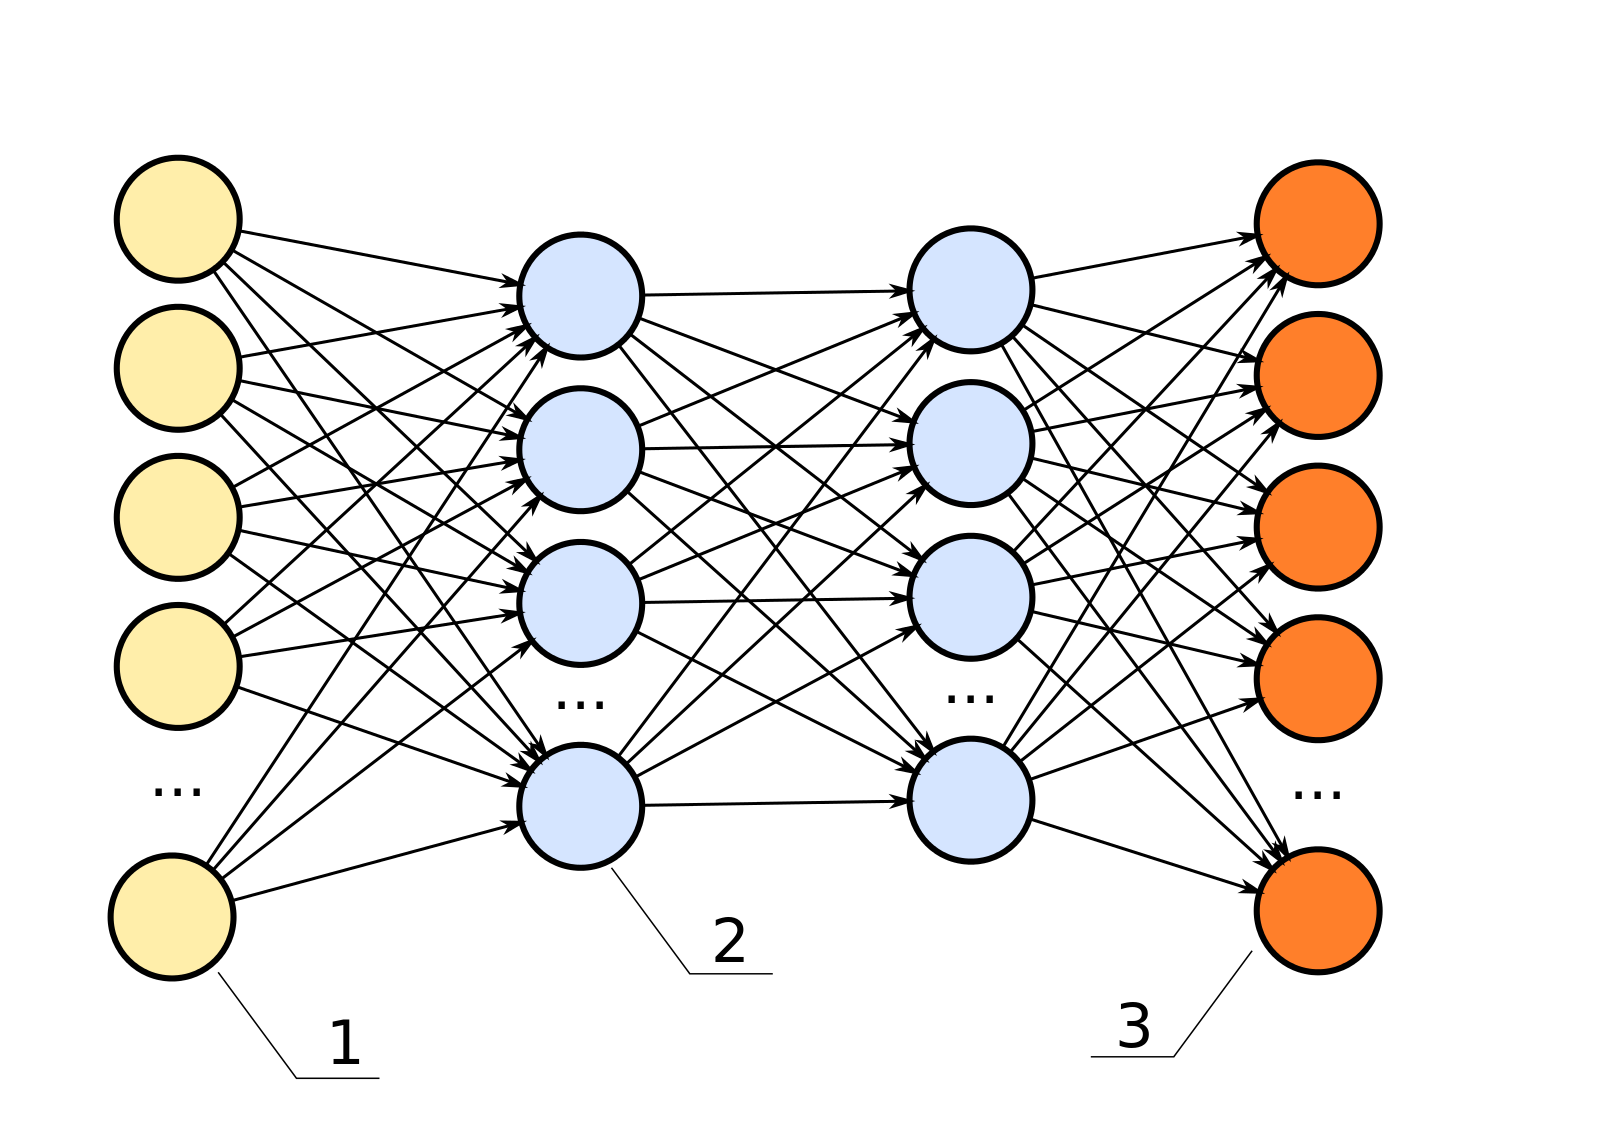
\includegraphics[width=7.5cm]{../pic/nn_example.png}\centering
	\end{center}
	
	Любую ЭС можно представить как нейронную сеть.
	
	Проблема нейронных сетей -- как их обучать.
\end{frame}

\begin{frame}{Backpropagation}
	Метод обратного распространения ошибки (backpropagation) 
	-- требует <<локальной связности>> признаков. 
	
	Изображение (пиксели), временные ряды, треки мыши, голос этой <<локальной связностью>>
	обладают.
	
	Текст естественного языка -- в меньшей степени. Но текстов очень много и букв всего 33.
\end{frame}

\begin{frame}{Проблема больших алфавитов и разряженных слов}
	
	Представьте себе цепочки с алфавитом в 300-500 букв,
	которые достаточно разряжены.
	
	TODO изображение.
	
	Теоретически их тоже можно решить нейронной сетью,
	однако потребуется большее количество данных, чем для текста.
\end{frame}


\section{Задача исследования активностей пользователей и мапинг.}\label{section:text_tasks}

\begin{frame}
		
	\begin{center}
		
\includegraphics[width=9.5cm]{../pic/sber_logo_1.png}\centering
	\end{center}

\end{frame}

\begin{frame}{Мапинг страниц}
	
\includegraphics[width=4.9cm]{../pic/sber_logo_1.png}
	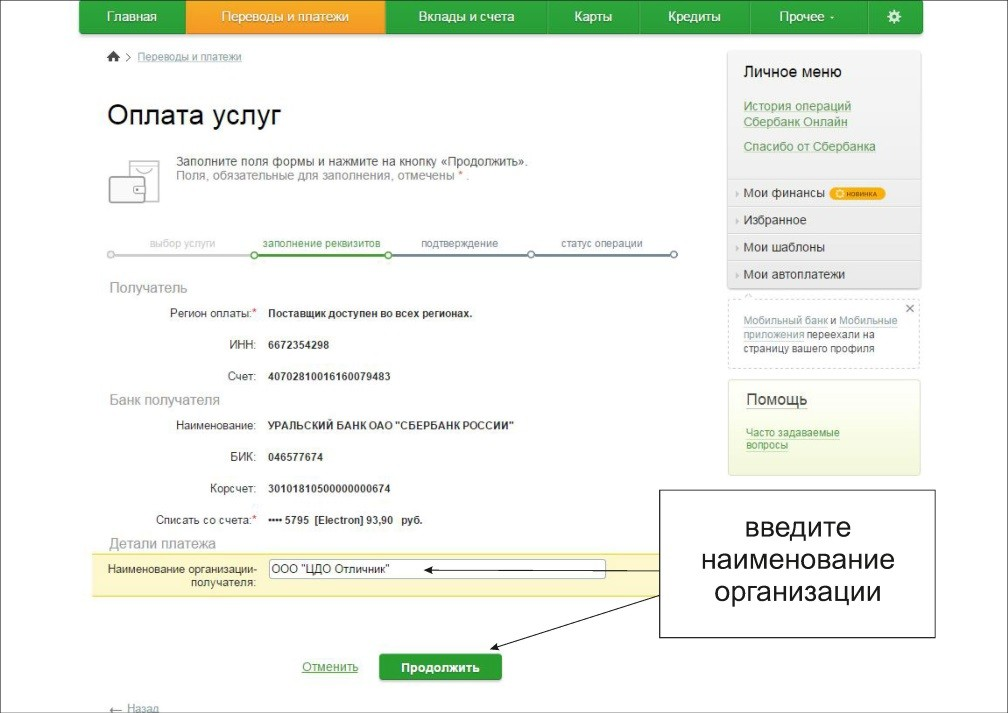
\includegraphics[width=5.7cm]{../pic/sber_logo_2.png}
	
	\textbf{https://[$\hat{}$/]+/CSAFront/index.do} ~~ $\longmapsto$ 258
	
	\textbf{https://[$\hat{}$/]+/PhizIC/private/payments/print.do$\backslash$?id=} ~~ $\longmapsto$ 54
\end{frame}

\begin{frame}{Мапинг страниц}
	Задача мапинга не тривиальна, как может показатся на первый взгляд.
	
	Одни из проблем мапинга:
	\begin{enumerate}
		\item Некоторые URL имеют таргетированную информацию (например номер счёта, id и т.д.).
		Эти числа не должны учитываться в регулярных выражениях.
		С другой стороны существуют существенные идентификаторы. 
		(В случае Сбербанк.Онлайн например ServiceID)
		\item Некоторые страницы делают одно и то же но в силу каких-либо исторических причин 
		имеют несколько url
		\item Приоритет регулярных выражений. Они могут пересекаться и возникнут ошибки.
		\item \auditorium{что ещё?}
	\end{enumerate}
\end{frame}

\begin{frame}{Построение мапинга}
	Процесс итеративный.
	\begin{enumerate}
		\item Собираем данные
		\item Пишем регулярные выражения
		\item Удаляем данные попавшие под регулярные выражения. Если ещё есть url, то goto 2
		\item goto 1
	\end{enumerate}
\end{frame}

\begin{frame}{SPA}
	Одностраничные приложения (single page application, SPA)
	имеют ровно один url
	
	\auditorium{Как проводим мапинг?}
\end{frame}

\

\begin{frame}{Итог мапинга}
	\small
	Любое нахождение на каком либо действии можно представить в виде действия.
	
	\begin{tabular}{lr}
		\textbf{regexp} & \textbf{num} \\
		... & ... \\
		https://[$\hat{}$/]+/PhizIC/private/payments/payment.do$\backslash$?id= & 50 \\
		https://[$\hat{}$/]+/PhizIC/private/payments/payment.do$\backslash$?template= & 51 \\
		https://[$\hat{}$/]+/PhizIC/private/payments/payment.do$\backslash$?offerId= & 52 \\
		... & ... \\
		https://[$\hat{}$/]+/PhizIC/private/news/dayList.do & 117 \\
		https://[$\hat{}$/]+/PhizIC/private/ima/office/list.do & 118 \\
	\end{tabular}
	
	Таким образом каждый url с помощью \textbf{regexp} мапится в уникальный 
	номер $num$ единственным способом. 
\end{frame}

\begin{frame}{Итог мапинга}
	С помощью мапинга любую  активность пользователя (сессию $S_i$)
	можно представить в виде последовательности
	действий:
	
	\begin{center}
		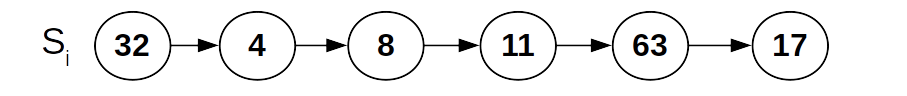
\includegraphics[width=11cm]{../pic/beh/chain.png}\centering
	\end{center}
\end{frame}

\section{Алгоритм behс}\label{section:behс}

\begin{frame}{Идея алгоритма}
	\small
	Существует набор различных сессий различных пользователей:
	\begin{center}
		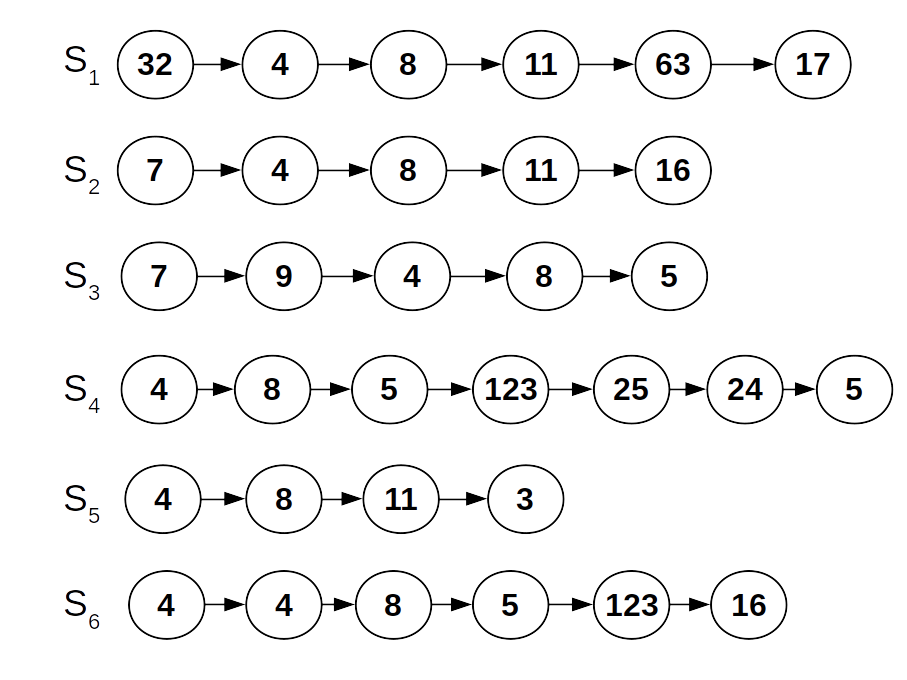
\includegraphics[width=10cm]{../pic/beh/idea_1.png}\centering
	\end{center}
\end{frame}

\begin{frame}{Идея алгоритма}
	\small
	Мы имеем маркировку, какие сессии мошеннические (feedback):
	\begin{center}
		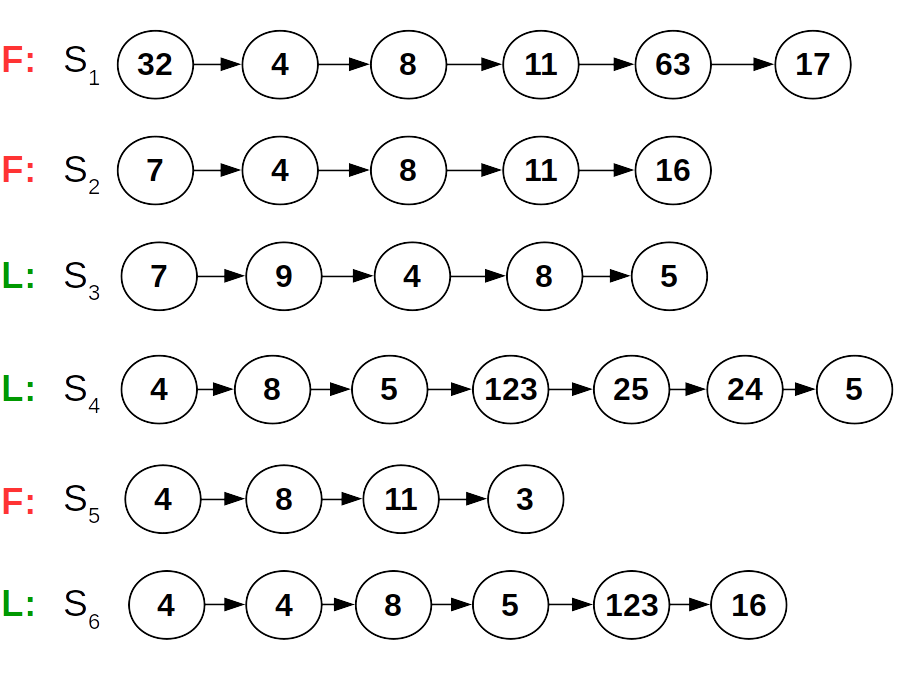
\includegraphics[width=10cm]{../pic/beh/idea_2.png}\centering
	\end{center}
\end{frame}

\begin{frame}{Идея алгоритма}
	\small
	Требуется Feature Extraction характерных \textit{подцепочек} для $F$ и $L$:
	\begin{center}
		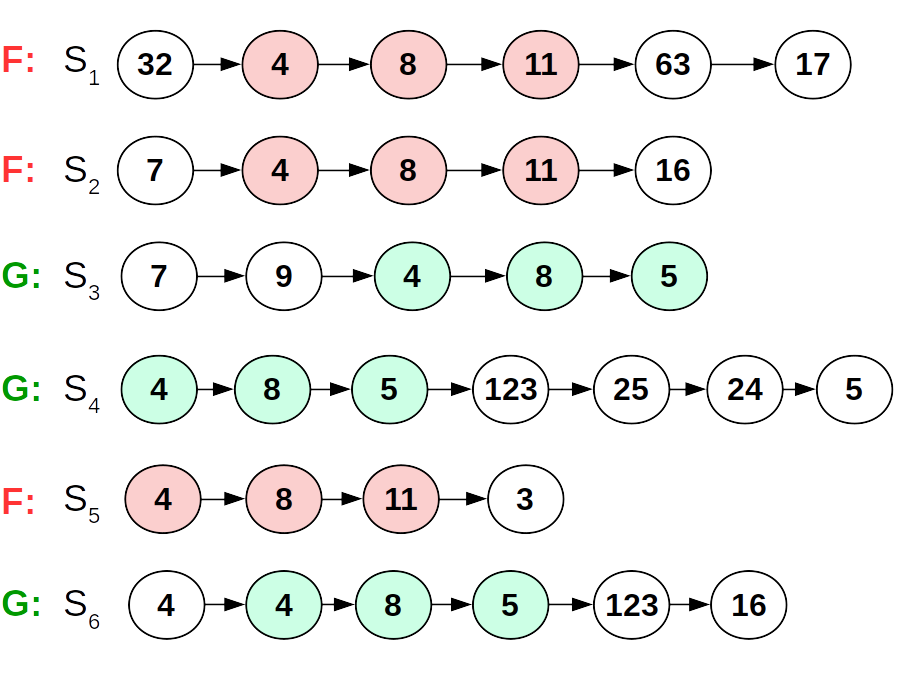
\includegraphics[width=10cm]{../pic/beh/idea_3.png}\centering
	\end{center}
\end{frame}

\begin{frame}
	\Large
	\centering
	\auditorium{Ваши предложения? \\ Как бы вы решали эту задачу?}
\end{frame}


% На этом слайде нужно рисовать маркером дерево переходов и объяснять как оно получилось
\begin{frame}[t]
	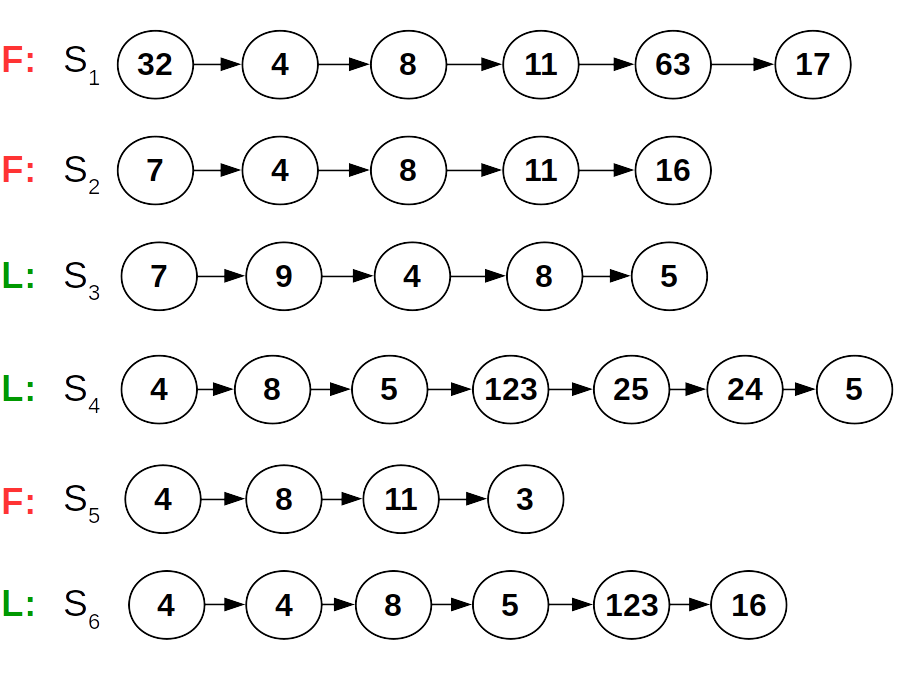
\includegraphics[width=5cm]{../pic/beh/idea_2.png}
\end{frame}

\begin{frame}
	\Large
	\centering
	Теперь давайте дадим \\ формальный алгоритм.
\end{frame}

\begin{frame}{Вес подпоследовательности}
	\small
	Любую сессию $S_i$ можно представить в виде
	\begin{equation}
	S_i = \left( s_1^i, s_2^i, ... s_n^i\right)
	\end{equation}
	при этом $n \neq const$, эта величина различна для разных $S_i$.
	
	Зафиксируем параметры $l_1$ и $l_2$.
	
	Введем операцию получения \textit{всех} подпоследовательностей $\bold b = (s_j^i, s_{j+1}^i, ...)$ длины $l_1 \leqslant l \leqslant l_2$
	из цепочки сессии $S_i$:
	\begin{equation}
	B(S_i ; l_1, l_2) = \left\{ \bold b \right\}_i
	\end{equation}
	
	Введём флаги:
	\begin{itemize}
		\item $f=0$ -- легитимная ($L$);
		\item $f=1$ -- мошенническая ($F$).
	\end{itemize}

	... ... ... ... ...
\end{frame}


\begin{frame}{Вес подпоследовательности}
	\small
	... ... ... ... ...
	
	Введем величину $C(\bold b, f)$, обозначающее количество $S_i$ из множества всех $\left\{ S_i \right\}$,
	которые содержат некий \textit{фиксированный} $\bold b$. 
	и которым соответствует некий фиксированный флаг $f$  
	
	На языке кванторов:
	\begin{equation}
	C(\bold b, f) \stackrel{def}{=} \lVert
		\left\{ 
			S_i \in  \left\{S_i\right\}   : \bold b \in S_i 
			\wedge f \longmapsto S_i
		\right\}
	\lVert
	\end{equation}
	
	Тогда для каждого $\bold b$ можно ввести два веса:
	\begin{equation}\label{eq:W_0_simple}
	W_0 (\bold b) \stackrel{def}{=} \frac{C(\bold b, 0)}{C(\bold b, 1) + 1}
	\end{equation}
	\begin{equation}\label{eq:W_1_simple}
	W_1 (\bold b) \stackrel{def}{=} \frac{C(\bold b, 1)}{C(\bold b, 0) + 1}
	\end{equation}
\end{frame}

\begin{frame}
	Введём \term{параметры} $C_0$ и $C_1$.
	
	Выберем $C_0$ подпоследовательностей $\bold b$ с максимальным весом $W_0$
	и $C_1$ подпоследовательностей $\bold b$ с максимальным весом $W_1$.
	
	Полученное множество -- и есть множество характерных подпоследовательностей.
	
	Feature Extraction завершён.

	\auditorium{В чём основная задача этого алгоритма? Что упустили? Неужели всё так просто?}	
\end{frame}
	
\begin{frame}
	Основная проблема алгоритма -- расчёт $C(\bold b, f)$. Для этого необходимо строить дерево переходов. 
	
	Введём операцию:
	\begin{equation}
	G(\bold b) = G\big( (s_1, s_2, ..., s_m) \big)
	= \big\{ (\lambda, s_1), (s_1, s_2), ... (s_{m-1}, s_m) \big\}
	\end{equation}
\end{frame}

\begin{frame}{Формальный алгоритм}
	\small
	\begin{enumerate}
		\item Определим $D$ как граф, содержащий ровно одну вершину $\lambda$.
		\item Выбираем любой $S_i$ из $\big\{ S_i\big\}$ и определяем флаг $f \longmapsto S_i$.
			\label{behc:item:get_next}
		\item \term{Помечаем} вершину $\lambda$.
		\item $\forall \bold b \in B(S_i; l_1, l_2)$:  
		$\forall (s_1, s_2) \in G(b)$: 
		\begin{enumerate}
			\item Если от \term{помеченной} $s_1$ нет
			вершины $s_2$, то создаём новую вершину $s_2$, ребро $s_1 \longmapsto s_2$,
			и для этого ребра устанавливаем вес $(c_0,c_1)=(0,0)$.
			\item Берём вес $\big(c_0, c_1\big)$ ребра $(s_1, s_2)$.
			Переопределяем вес:
			\begin{enumerate}
				\item $\big(c_0 + 1, c_1\big)$, если $f=0$;
				\item $\big(c_0, c_1 +1 \big)$, если $f=1$.
			\end{enumerate}
			\item \term{помечаем} вершину $s_2$.
		\end{enumerate}
		\item Удаляем $S_i$ из множества $\big\{ S_i\big\}$.
		\item Если $\big\{ S_i\big\}\neq \varnothing$, то переходим на п.\ref{behc:item:get_next}.
		\item Проходим по дереву и рассчитываем все $C(\bold b, f)$
		через рёбра дерева. Рассчитываем все $W_0(\bold b)$ и $W_1(\bold b)$.
	\end{enumerate}	
\end{frame}

\begin{frame}{Пример. Вход}
	\centering
	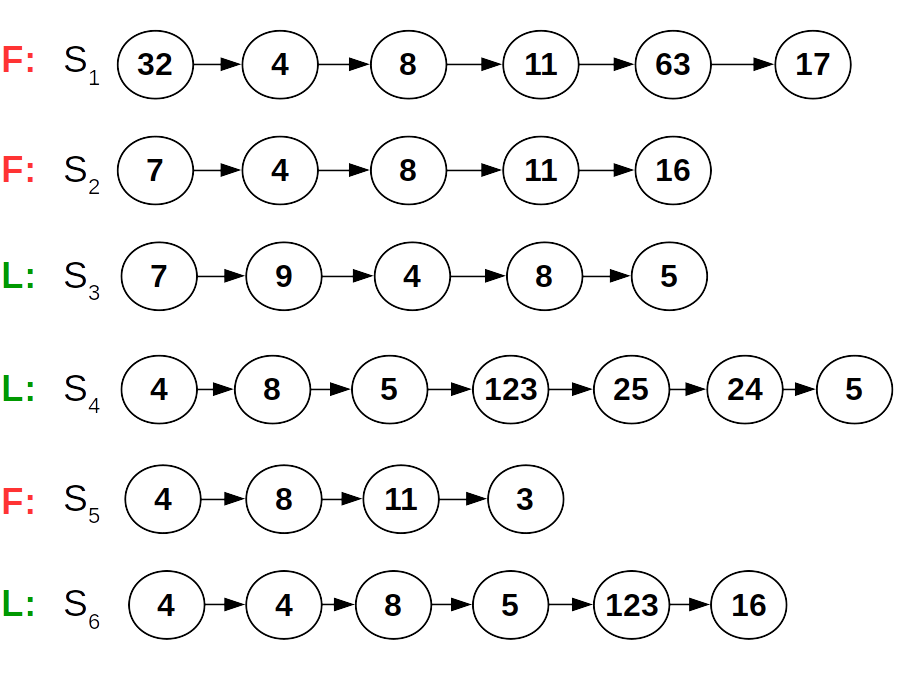
\includegraphics[width=11cm]{../pic/beh/idea_2.png}
\end{frame}

\begin{frame}{Пример. Выход}
	% TODO перерисовать D_example.odg полностью!
	\centering
	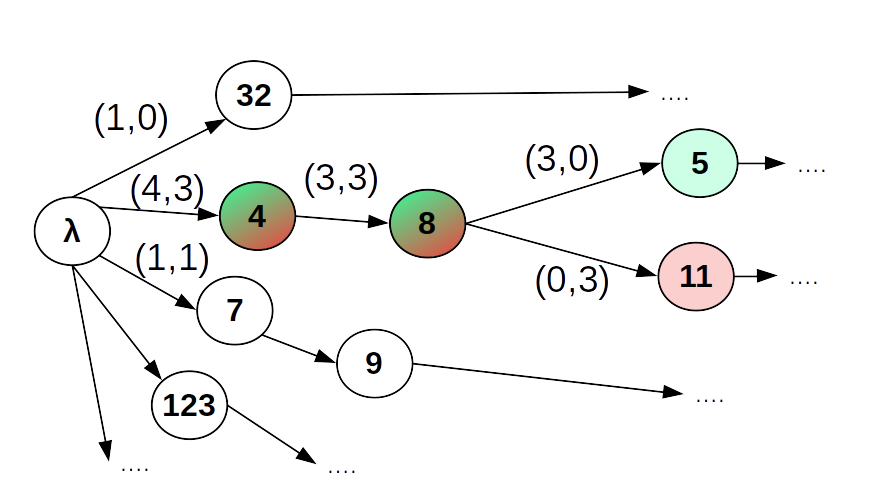
\includegraphics[width=11cm]{../pic/beh/D_example.png}
\end{frame}

\begin{frame}{Пример. Выход}
	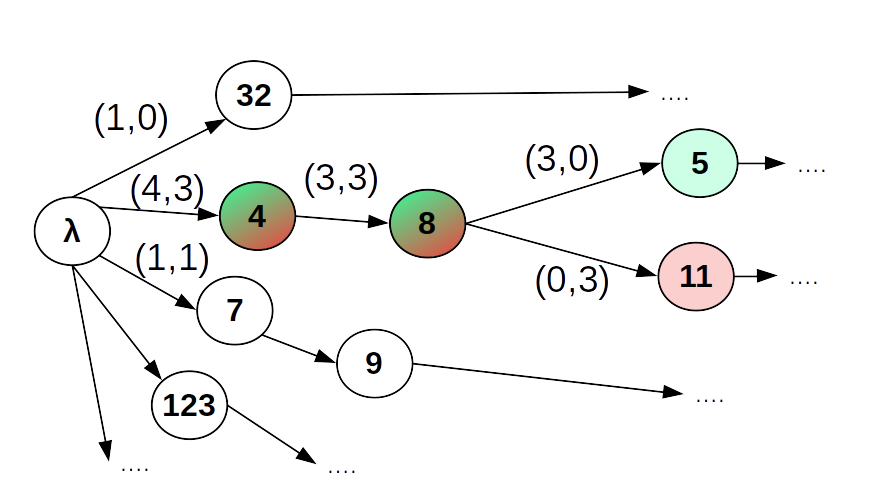
\includegraphics[width=8cm]{../pic/beh/D_example.png}
	
	В этом примере:
	\begin{itemize}
		\item $C \big( (4,8); 0\big) =  C \big( (4,8); 1\big) = 3$;
		\item $C \big( (4,8,5); 0\big) = 3$, $C \big( (4,8,5); 1\big) = 0$;
		\item $C \big( (4,8,11); 0\big) = 0$, $C \big( (4,8,11); 1\big) = 3$.
	\end{itemize}
	
\end{frame}


\begin{frame}{Важные нюансы}
	Существует проблема <<похожих>> подпоследовательностей.
	Это когда их длина отличается на 1, но у них примерно похожие $W_1$ или $W_2$.
	Таким образом они обе попадут в признаки. \auditorium{Что делать?}
	
	Формулы \eqref{eq:W_0_simple} и \eqref{eq:W_1_simple} не являются оптимальными 
	и плохо работают когда $C(\bold b, 0)$ и/или $C(\bold b, 1)$ малы.
	\auditorium{Как решаем эти проблемы?}
	
	И самое важное: алгоритм не учитывает корреляцию цепочек друг с другом. 
	Однако на практике как правило это не существенно. \auditorium{Почему?}
\end{frame}








\section{Алгоритм behi}\label{section:behi}


\section{Вопросы для самопроверки}

\end{document}